\pagebreak

\section{Dameaften}
\subsubsection*{\textbf{Ansvarlige:} \Randildo \& \Karla}

\textbf{Sted:} Pejsestuen \\

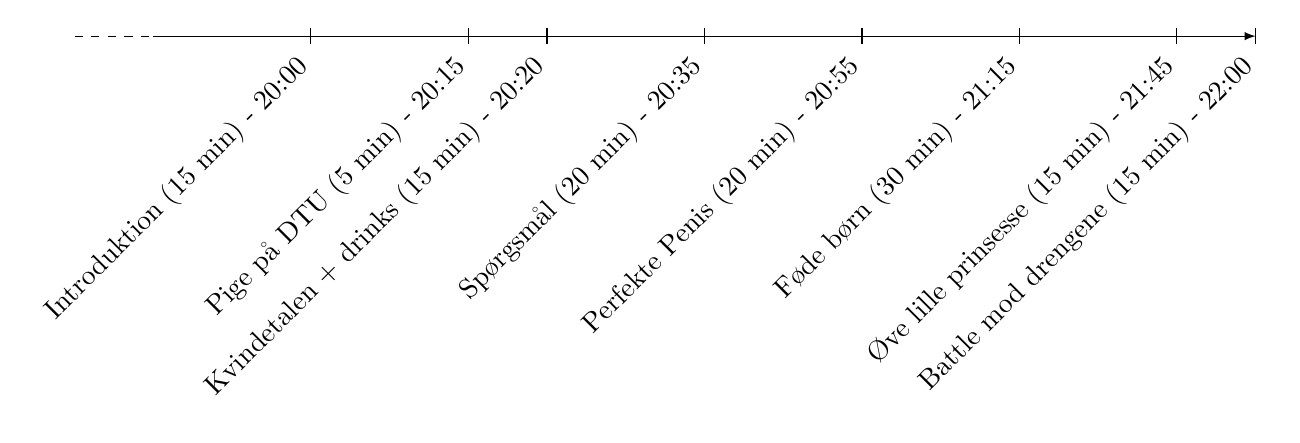
\begin{tikzpicture}
   \draw[-, dashed] (-1,0) -- (0,0);
   \draw[|->, -latex] (0,0) -- (14,0);
   
   \draw[] (2,-0.1) -- (2,0.1);
   \draw (2,0) node[below=7pt,anchor=east,xshift=0,rotate=45] {Introduktion (15 min) - 20:00}; 
   
   \draw[] (4,-0.1) -- (4,0.1);
   \draw (4,0) node[below=7pt,anchor=east,xshift=0,rotate=45] {Pige på DTU (5 min) - 20:15}; 
   
   \draw[] (5,-0.1) -- (5,0.1);
   \draw (5,0) node[below=7pt,anchor=east,xshift=0,rotate=45] {Kvindetalen + drinks (15 min) - 20:20}; 
   
   \draw[] (7,-0.1) -- (7,0.1);
   \draw (7,0) node[below=7pt,anchor=east,xshift=0,rotate=45] {Spørgsmål (20 min) - 20:35};
   
   \draw[] (9,-0.1) -- (9,0.1);
   \draw (9,0) node[below=7pt,anchor=east,xshift=0,rotate=45] {Perfekte Penis (20 min) - 20:55};

   \draw[] (11,-0.1) -- (11,0.1);
   \draw (11,0) node[below=7pt,anchor=east,xshift=0,rotate=45] {Føde børn (30 min) - 21:15};
   
   \draw[] (13,-0.1) -- (13,0.1);
   \draw (13,0) node[below=7pt,anchor=east,xshift=0,rotate=45] {Øve lille prinsesse (15 min) - 21:45}; 
   
   \draw[] (14,-0.1) -- (14,0.1);
   \draw (14,0) node[below=7pt,anchor=east,xshift=0,rotate=45] {Battle mod drengene (15 min) - 22:00}; 
\end{tikzpicture}

\subsection*{Introduktion}
Start: 20:00 \\
Tid: 15 minutter \\
Velkommen til pigeaften. Her skal vi bare hygge os helt vildt meget. Vi starter lige med en navnerunde hvor i kan fortælle lidt om jer selv:
\begin{itemize}
  \item Navn
  \item By
  \item Yndlings drink
  \item Fact om en selv
\end{itemize}

\subsection*{Pige på DTU}
\subsubsection*{\textbf{Ansvarlige:} \Karla}
Start: 20:15 \\
Tid: 5 minutter \\
Kære piger. \\
Jeg kan ikke forestille mig andet end at der i gymnasiet – eller hvor I ellers gik - skete rigtig mange ting; I udviklede jer selvfølgelig fagligt, men I lærte også meget om jer selv og menneskerne omkring jer. Det vil også ske på DTU. Det vil virkelig gøre mig glad, hvis det lykkes os at give jer den bedst mulige start på alle de her nye ting. Vi har jo været i gennem meget af det samme, så brug os, spørg os til råds om hvad end I har på hjertet. For der sker meget nyt. \\
Én af de ting I skal være forberedt på, og som sandsynligvis vil være nyt for de fleste af jer, er det markante overtal af drenge, I hele tiden vil være omgivet af. Og I kender dem – de kan sku godt være lidt liderlige og være det lidt hele tiden. Så tænk på jeres ry. I skal ikke blive skræmt, tage kyskhedsbælte på og smide nøglen væk, men de fleste af jer skal sandsynligvis være her i fem år, så pas på jer selv. Der kommer massere af muligheder for at slå jer løs. (Det gælder om at være glad i det lange løb :-) ).

\subsection*{Kvindetalen + drinks}
\subsubsection*{\textbf{Ansvarlige:} \Randildo}
Start: 20:20 \\
Tid: 15 minutter \\
Der serveres drinks inden talen begynder. \\

\subsection*{Spørgsmål}
Start: 20:35 \\
Tid: 20 minutter \\
Hver rus får en hvid serviet og en grøn serviet. Hvid serviet er negativ, grøn serviet er positiv. Servietten rækkes i vejret som svar på spørgsmålene som vektorerne stiller.

\begin{itemize}
  \item Hvem har en kæreste?
  \item Hvem har bare en lækker mand?
  \item Hvem har et sted at bo?
  \item Hvem kan godt lide at gå i kjoler?
  \item Hvem kan ridde?
  \item Hvem har malket en ko?
  \item Hvem har gået på STX?
  \item Hvem har gået på HTX?
  \item Hvem kan lave en fransk fletning?
  \item Hvem har været på en andet kontinent?
  \item Hvem har haft et sabbatår?
  \item Hvem kommer fra Jylland?
  \item Hvem kommer fra Sjælland?
  \item Hvem kommer fra Fyn?
  \item Hvem kan slikke på deres egen nipple? (prøv hvis stemningen er til det)
  \item Hvem har været sammen med deres kæreste i mere end 2 år?
  \item Var det nemt at finde kostume?
  \item Hvem er til storbyferie?
  \item Hvem er til badeferie?
  \item Hvem er til aktive ferier?
  \item Hvem er romantikere?
  \item Bliver mænd lækrere i jakkesæt? (glæd jer til årsfest)
\end{itemize}

\subsection*{Den perfekte penis}
Start: 20:55\\
Tid: 20 minutter\\
Introduktion: \randildo
Man får en klump trylledej hver og skal forme den perfekte penis.\\
Vi bruger den samme trylledej som fra natløbet mandag.\\

\subsection*{Føde børn}
Start: 21:15 \\
Tid: 30 minutter \\
Introduktion af \hspace{.1em} \Hyttebums{Jack}og\hspace{.2em} \Hyttebums{Turn-On} \\
Man ligger som om man skal føde, har en cykelslange mellem benene og skyder en bamse af sted. En anden pige står for at gribe den mellem armene som en jordmoder. 

\subsection*{Øve lille prinsesse}
Start: 21:45 \\
Tid: 15 minutter \\
Øve lille prinsesse efter sangbogen samt finde på flere vers, så vi kan slå drengene. Pigerne vinder.

\subsection*{Lille prinsesse – battle mod drengene}
Start: 22:00 \\
Tid: Så lang tid den kan fortsættes \\
Battle mod drengene i lille prinsesse. \\
Pigerne skal vinde (have skrevet nogen på forhånd)
\begin{itemize}
  \item Jeg kan dig ikke føle
  \item Du kom jo alt for hurtigt
  \item Din bror var 3 gange større
  \item Hvis der kommer noget om søster: hun er jo længe afdød
  \item Gå hjem til plastikdukken
  \item Behøver jeg sige mere
\end{itemize}

\subsection*{Materialeliste:}
\begin{itemize}
  \item Hvide servietter
  \item Grønne servietter
  \item 2-3 Cykelslanger
  \item 2-3 Bamse-lignende ting
  \item 6L danskvand
  \item 1 flaske Hyldeblomstsaft
  \item 6 lime
  \item 2 flaske vodka
\end{itemize}

\pagebreak
Ærede kvinder, mine Damer! \\
Vi er her samlet her i dag som ligesindede, \underline{\textbf{UDEN MÆND}}. Og hvorfor er vi det? Det er vi fordi vi har en historisk pligt til at samles for at praktisere én af den uendelige mængde af ting, som vi kvinder gør bedre end mænd. Og hér snakker jeg ikke om evnen til at dufte godt, være syg uden at klynke, rydde op i køkkenet UNDER madlavning eller utallige andre kompetencer såsom evnen til at koncentrere sig i længere tid. Jeg taler heller ikke om evnen til at lave en matematikaflevering, mens vi taler i telefon og samtidig får klaret dagens knibeøvelser. Nej, jeg snakker om evnen til at diskutere \textbf{VIGTIGE TING!} I år 0 blev det lille Jesus barn født af ingen ringere end selveste Jomfru Maria; En fantastisk kvinde, hun klarede det hele selv, \underline{\textbf{UDEN MÆND}}. Men hvordan gjorde hun det? Jo, hende og Gud havde diskuteret \textbf{VIGTIGE TING!} Mændenes historie fyldt med blod, og meningsløs vold og død. Det var aldrig gået så galt, hvis blot vi havde levet \underline{\textbf{UDEN MÆND!}} Eksemplerne er talrige: Alexander den Stores erobringstogt i år 336 f. kr., Hunnerkongen Attilas togt i 430 med plyndring og voldtægt, Vikingerne, Napoleon, Stalin, Hitler. Alle disse timer og liv spildt, blot fordi mænd ikke kan finde ud af at diskutere \textbf{VIGTIGE TING!} Snakker vi derimod kvindelige regenter, så har der, for hver eneste konge igennem historien været en dronning ved hans side, men når man kigger nøje efter vil man opdage, at der ikke for hver dronning har været en konge! Jeg taler om Kleopatra, Elizabeth I og selvfølgelig om Danmarks to Margrether’; Dronninger som har formået at samle Norden, lede Nationen og regere over folket og de har gjort det \underline{\textbf{UDEN MÆND}}. Men hvordan gjorde de det? Ved at diskutere \textbf{VIGTIGE TING!} På trods af, at mændene dræber og kvinderne skaber, så er det alligevel mændenes bedrifter som har fået størst genklang i historien. Derfor vil vi i dag gerne ære to kvinder, som er blevet overset, men som har banet vejen for, at vi sidder her i dag, nemlig: Agens Klingberg og Betzy Meyer, der i 1897 blev Danmarks første kvindelige ingeniører. Det gjorde de \underline{\textbf{UDEN MÆND, PÅ TRODS AF MÆND}} og de gjorde det ved at diskutere \textbf{VIGTIGE TING!} Når mænd mødes, uden kvinder, så bruger de tiden på at diskutere ting såsom, hvis prut der lugter mest, hvem der er kommet længst i Command and Conquer, hvem der har håneretten i ølrisk eller hvem der er den bedste James Bond. Er det vigtige ting? (\textbf{NEJ!}) Vi kvinder sidder IKKE og klør os i skridtet, piller næse og finder navlefnuller uden at kunne overskue at rejse os op for at hente en bajer, \textbf{NEJ!}, når kvinder mødes, \underline{\textbf{RIGTIGE KVINDER}}, nøjagtigt som vi gør her i aften og som vi vil mødes i al fremtid, bliver relationer skabt, verdenssituationen vendt, problemer løst, skønhed udforsket og viden delt! Der bliver sammenlignet outfits, snakket om penislængder, og analyseret sms’er. Men først og fremmest så bliver der diskuteret.. \textbf{VIGTIGE TING! VIGTIGE TING! VIGTIGE TING!}

\pagebreak
